\section{Approach}\label{sec:approach}

Beginning with SKLearn~\cite{scikit-learn} data readiness was proven with moderately successful classification using
a simple SVM and then the SKLearn Multi-Layer-Perceptron neural network, getting 70-80\% accuracy, well above the
random chance accuracy of 50\%, sufficing the
initial sanity check that deep learning would be ready to work on.

% TODO these are relevant citations, right?
Leveraging PyTorch~\cite{paszke2017automatic} first a framework for learning was likewise vetted using a simple fully
connected shallow network, graduating to the state of the art convolutional networks, chiefly focussed
on the ResNet~\cite{he2016deep} architecture styles, which have been developed for video classification~\cite{tran2018closer}
utilizing 3 dimensional convolutions much in the way 2 dimensional convolutions operate, which have
been shown to hold a slight edge on 2 dimensions~\cite{payan2015predicting} in other applications.


\subsection{Data Preparation}\label{subsec:data-preparation}

First as the data was not prepared for classification, critical cleaning include subtracting the mean image to better
highlight meaningful variance, and standardizing the data between 0 and 1.

Given the nature of the input images being 3d brain scans it's intuitive that examining the brain in 3 dimensions
allows for much more interesting patterns of brain activity and structuring being recognized.

This comes with a substantial cost however, as the extra dimension explodes the memory demands of the input data, and
the number of trainable parameters for the models.
Many of the recommendations following will vary based on the particular hardware, but with a 4GB GPU I had to be quite
careful about batch-sizes to not over-allocate memory.
To combat this, first, a relatively conservative amount of blank space is cropped from the images, halving the total footprint.
Following this, in order to use a batch-size of 64, I interpolate images to approximately $\frac{5}{6}$ their original dimension

In addition, I typically do not use the full cohort of 30 subjects, as I even encounter some RAM restrictions with the
full raw dataset consisting of
$64 sagital \times 64 coronal \times 30 axial \times 1 channel \times 32bit floats \times 375 scans \times 30 subjects$ or roughly 5.53 gigabytes

In working with 2 dimensions, omitting the axial dimension for a flat cross section, you'll see the dataset is
$\frac{1}{30}$ the size and hence, much more manageable.


\subsection{Examining the Data}\label{subsec:examining-data}

Two fully processed, correctly classified brain scans are presented in the figure~\ref{fig:comparison}
which pose a daunting challenge to human labelers.


\begin{figure}
  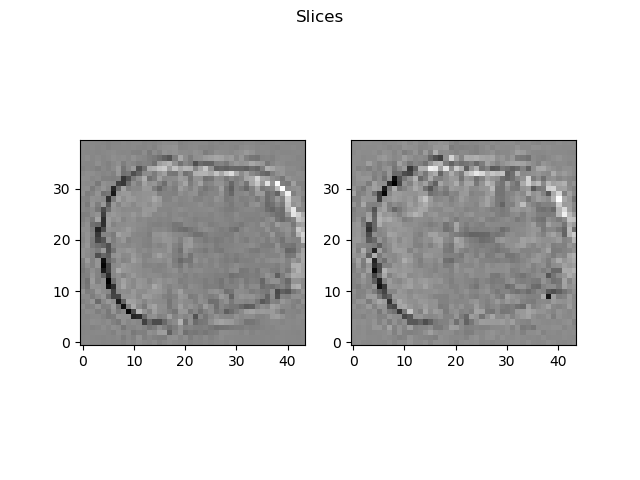
\includegraphics[width=\linewidth]{images/nf_f_hard_comparison.png}
  \caption{Nonfood-Stimuli \& Food-Stimuli Respectively from the same Subject}
  \label{fig:comparison}
\end{figure}

\subsection{Model Selection}\label{subsec:model-selection}

For the primary focus of comparing and improving classification accuracy using 2d and 3d architectures, ResNet models
of the standard 18 layers to 100+ layers are examined, as the ResNet family is both highly competitive, and demonstrated
in both 2 and 3 dimensions which will help comparisons in exploring the benefits of 3d brain scan usage.
Video processing typically limits the layers to a more shallow level than that of image processing, as unfortunately as
with the data, the model parameters explode out of control pretty fast, though some have seen minor improvements by
going deeper~\cite{hara3dcnns}.
The following parameter counts are from standard ResNet architectures adapted to a single input channel.

\begin{center}
 \begin{tabular}{||c c c||}
 \hline
 - & ResNet-18 2d & ResNet-18 3d \\ [0.5ex]
 \hline\hline
 Counts & 11,171,266 & 33,148,482 \\ [1ex]
 \hline
 Ratio & 1.0 & 2.97 \\ [1ex]
 \hline
\end{tabular}
\end{center}

\subsection{Comparisons}\label{subsec:comparisons}

Model performance is typically evaluated using accuracy, precision, recall, and AUC metrics, as well as total time to
train.
